\begin{pastexam}[label={px:ncku-107-prog-03}]{成大資訊聯招 107 學年度 第 3 題}
（填表）

(10\%) Please write down the adjacency matrix of the following graph in the following table.

\begin{center}
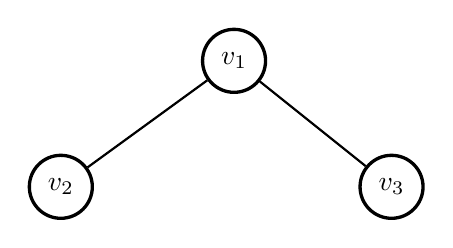
\begin{tikzpicture}[v/.style={circle,draw,very thick,inner sep=1pt,minimum size=8mm},thick]
\node[v] (1) at (2.2,1.6) {$v_1$};
\node[v] (2) at (0,0) {$v_2$};
\node[v] (3) at (4.2,0) {$v_3$};
\draw (1) -- (2);
\draw (1) -- (3);
\end{tikzpicture}

\vspace{6pt}
\begin{tabular}{|c|c|c|c|}
\hline
 & $v_1$ & $v_2$ & $v_3$ \\ \hline
$v_1$ & \hspace{2em} & \hspace{2em} & \hspace{2em} \\ \hline
$v_2$ & & & \\ \hline
$v_3$ & & & \\ \hline
\end{tabular}
\end{center}
\end{pastexam}

\begin{pastsoln}
答案：
\begin{center}
\begin{tabular}{|c|c|c|c|}
\hline
 & $v_1$ & $v_2$ & $v_3$ \\ \hline
$v_1$ & 0 & 1 & 1 \\ \hline
$v_2$ & 1 & 0 & 0 \\ \hline
$v_3$ & 1 & 0 & 0 \\ \hline
\end{tabular}
\end{center}

鄰接矩陣（資結書第~21.2~節）是 $n \times n$ 的表，第 $i$ 列第 $j$ 欄填 $1$ 表示有邊 $(v_i, v_j)$，
填 $0$ 表示沒有。 圖上的線沒有箭頭，是無向圖，邊有 $\{v_1, v_2\}$、$\{v_1, v_3\}$ 兩條。
\begin{itemize}
\item 每條無向邊在矩陣裡出現兩次：$\{v_1, v_2\}$ 填在 $(1,2)$ 和 $(2,1)$，$\{v_1, v_3\}$ 填在
$(1,3)$ 和 $(3,1)$。 所以矩陣對稱。
\item $v_2$、$v_3$ 之間沒有邊，$(2,3)$、$(3,2)$ 是 $0$。
\item 沒有自環，對角線全是 $0$。
\end{itemize}
檢查：每一列的和是那個頂點的度數，$v_1$ 是 $2$、$v_2$ 和 $v_3$ 是 $1$；全部加起來 $4 = 2 \times 2$，
是邊數的兩倍（握手定理）。
\end{pastsoln}
